\documentclass[12pt]{article}
\usepackage{amsmath}
\usepackage[margin=1 in]{geometry}
\usepackage{graphicx}
\usepackage{booktabs}
\usepackage{natbib}
\usepackage{lipsum}
\usepackage[colorlinks=true, citecolor=blue]{hyperref}

\title{Stats Paper}
\author{Jessica Zambuto\\
Department of Statistics, University of Connecticut}

\begin{document}
\maketitle

\begin{abstract}
Input abstract info 	
\end{abstract}

\section{Introduction}
\label{sec:intro}

\lipsum[1-3]
To cite a reference, here are examples.
\citet{xie2015dynamic} did something ... \lipsum[1]

A lot of work has been done \citep[e.g.,][]{xie2015dynamic}.
\lipsum[2]

\section{Data}
\label{sec:data}
\begin{equation}
  \label{eq:mc2}
  E= m c^2
\end{equation}
\lipsum{1}


\section{Methods}
\label{sec:meth}
\begin{equation}
	\label{eq:area}
	\pi r^2
\end{equation}
Equation~\eqref{eq:area} is the area of a circle.
An unnumbered equation looks like:
\[
f(x)=\frac{1}{\sqrt{3\pi}}\exp
\]

\section{Results}
\label{sec:results}
Table~\ref{tab:rv} summarizes some example draws from some distributions.
\lipsum[1-4]

\begin{table}[ht]
  \caption{This is my first table.}
  \label{tab:rv}
\centering
\begin{tabular}{rrr}
  \toprule
normal & poisson & gamma \\ 
  \midrule
-0.110 & 4 & 2.401 \\ 
  0.116 & 4 & 3.529 \\ 
  -0.828 & 9 & 2.112 \\ 
  -0.066 & 6 & 11.104 \\ 
  0.219 & 3 & 4.815 \\ 
  0.303 & 5 & 2.188 \\ 
  0.544 & 0 & 8.050 \\ 
  -2.617 & 8 & 3.646 \\ 
  0.747 & 1 & 5.178 \\ 
  -1.103 & 4 & 3.043 \\ 
   \bottomrule
\end{tabular}
\end{table}

Figure~\ref{fig:cars} shows the distance against the speed from this dataset.

\begin{figure}
  \centering
  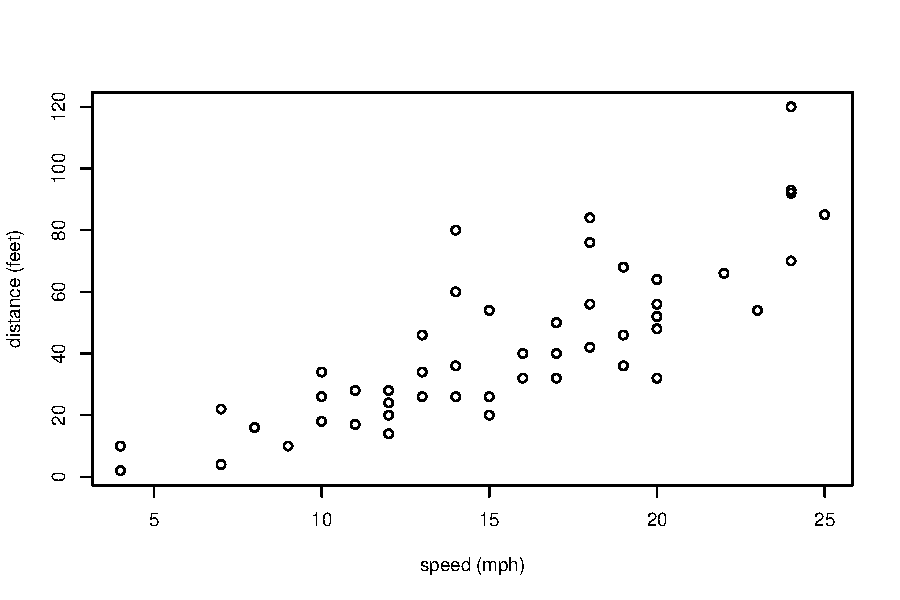
\includegraphics[width=\textwidth]{cars.pdf}
  \caption{This is my first figure.}
  \label{fig:cars}
\end{figure}

\section{Discussion}
\label{sec:disc}

\bibliography{refs}
\bibliographystyle{chicago}

\end{document}

